\chapter{Introduction}

\section{Project Assignment}

The scope of this project is to perform a static analysis of the Clang compiler source code available at
\url{https://llvm.org/}, \url{https://clang.llvm.org/}.
In details, the project consists in:
\begin{itemize}
	\item Analyze the C/C++ source code for the Clang project, using different tools for static analysis. The
minimum number of tools that shall be selected is 2, and mandatorily it shall be used Understand++ and Clang static analyzer.
	\item Discuss the output of the different tools and their performance.
\end{itemize}
Some possible tools for static analysis are:
\begin{itemize}
	\item Understand++ \url{https://scitools.com/student/}
	\item SonarCube \url{https://www.sonarqube.org/}
	\item Cert C Rosechecker (also available pre-installed in a Virtual Machine) \url{https://www.cert.org/secure-coding/tools/rosecheckers.cfm}
	\item Clang static analyzer
	\item Cppcheck
	\item Many others can be retrieved from:
	\begin{itemize}		
	 	\item[ - ]\url{https://www.owasp.org/index.php/Source_Code_Analysis_Tools}
		\item[ - ]\url{https://en.wikipedia.org/wiki/List_of_tools_for_static_code_analysis\#C,_C++}
	\end{itemize}
\end{itemize}

Depending on the characteristics of the selected tool, it is recommended to comment on:
\begin{itemize}
	\item the output of the static analyzers with respect to the computed metrics,
	\item compliance to coding rules as MISRA, CERT C, ISO/IET 17961,
	\item correct/missed/false detection.
\end{itemize}

It is recommended to compare the output of the tools with the information that is already available about
the source code and provided by the developers, especially in terms of existing weaknesses of the software.

\section{Overview}

The scope of this work is to analyze the Clang compiler with a set of static analysis tools, in order to detect violations to standards and to common coding rules (such as MISRA) and security weaknesses such as the ones pointed in the CWE (Common Weaknesses Enumerator).\newline\newline
Several tools were used for this purpose:
\begin{itemize}
	\item Understand
	\item Clang Static Analyzer
	\item CppChecker
	\item Flawfinder
	\item Sonarqube
	\item Rosechecker
\end{itemize}
Unfortunately, not all of them were applicable for this work, due to the complexity of the project's architecture or the inflexibility of the tool.\newline
After collecting the results, these were then compared in terms of:
\begin{itemize}
	\item Violations found
	\item Performances
	\item Rules used to detect violations
	\item Easiness of the tool
\end{itemize}
\section{Static Analysis}
Static Analysis is a technique used to analyze softwares without actually executing them.\newline
In general this methodology relies on tools that inspect the source code in order to detect violations with respect to a set of well-defined rules. These tools usually operate by checking the syntax of the code, the semantic, the execution flow\dots \newline\newline
There are several advantages when adopting this technique:
\begin{itemize}
	\item First of all, by checking the actual source code, it is possible to identify the direct cause of a vulnerability/bug
	\item If it is used during the design/development process of a software, it improves its cleanness and correcteness
	\item The analysis is done with (almost) zero interactions by the human operator
\end{itemize}

The tools used to perform an analysis can be distinguished with respect to the phase in which the analysis is performed:

\begin{itemize}
	\item Unit Level
	\begin{itemize}
		\item[$\rightarrow$] The analysis takes place within a specific program (or a part of it) without taking into account interactions with other programs
	\end{itemize}
	\item Technology Level
	\begin{itemize}
		\item[$\rightarrow$] Analysis takes into account the interactions between unit programs, having a more general overview of a project
	\end{itemize}
	\item System Level
	\begin{itemize}
		\item[$\rightarrow$] The analysis consider the interaction between unit programs but without being limited to a specific technology
	\end{itemize}
	\item Business Level
	\begin{itemize}
		\item[$\rightarrow$] The analysis also takes into account aspects related to business processes implemented in the software system
	\end{itemize}
\end{itemize}

In our work we are interested in \textbf{Unit Level Analysis}.
\pagebreak

\section{LLVM-Clang Compiler}

The LLVM compiler infrastructure project is a "collection of modular and reusable compiler and toolchain technologies" used to develop compiler front ends and back ends \cite{bibitem1}. It is a middle-layer between the frontend (C, C++, Python\dots code) and the backend (low-level hardware-dependent assembly). The high-level source code is translated into \textsl{LLVM bitcode}: an intermediate language (such as the JVM bytecode) where optimization and analysis is performed before being translated to low-level code.\newline
The Clang compiler is a C/C++ (and several others) compiler frontend that uses the LLVM infrastracture. 
The project is structured in a complex hierarchy of directories and files, referencing each others. This was one of the two reasons that forced us to work on a sub-part of the project: the \textbf{tools/libclang} directory. The other reason was that some files made some of the static analyzers crash in unexpected manners, probably because of some sort of overflow.\newline\newline
\begin{minipage}{\linewidth}
	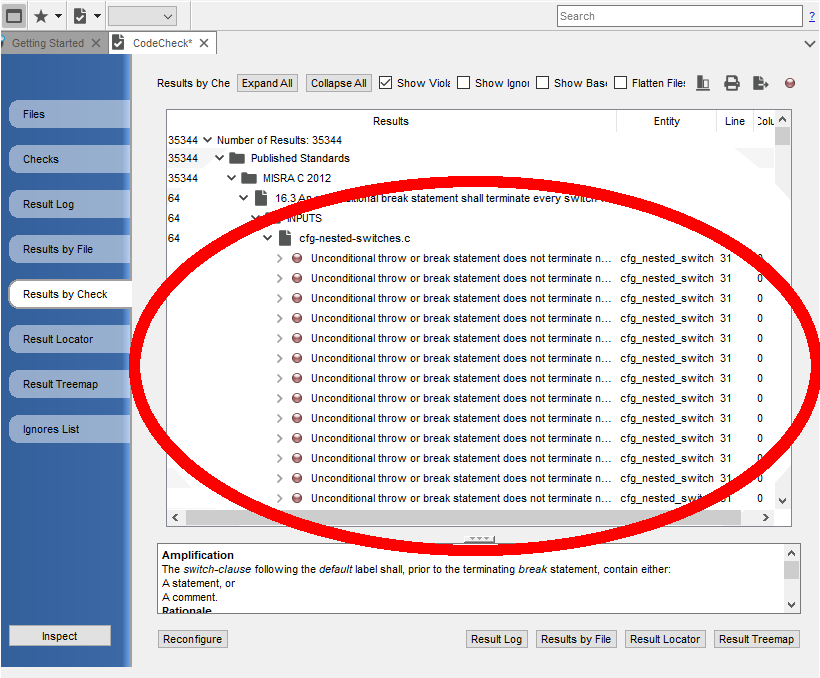
\includegraphics[width=\textwidth]{img/overflowUnderstand.png}
	\captionof{figure}{As we can see from this example, the same warning is displayed multiple times. This is most likely an overflow bug on the specific check}
\end{minipage}

